\documentclass[11pt,]{article}
\usepackage{lmodern}
\usepackage{amssymb,amsmath}
\usepackage{ifxetex,ifluatex}
\usepackage{fixltx2e} % provides \textsubscript
\ifnum 0\ifxetex 1\fi\ifluatex 1\fi=0 % if pdftex
  \usepackage[T1]{fontenc}
  \usepackage[utf8]{inputenc}
\else % if luatex or xelatex
  \ifxetex
    \usepackage{mathspec}
    \usepackage{xltxtra,xunicode}
  \else
    \usepackage{fontspec}
  \fi
  \defaultfontfeatures{Mapping=tex-text,Scale=MatchLowercase}
  \newcommand{\euro}{€}
\fi
% use upquote if available, for straight quotes in verbatim environments
\IfFileExists{upquote.sty}{\usepackage{upquote}}{}
% use microtype if available
\IfFileExists{microtype.sty}{%
\usepackage{microtype}
\UseMicrotypeSet[protrusion]{basicmath} % disable protrusion for tt fonts
}{}
\usepackage[margin=1in]{geometry}
\ifxetex
  \usepackage[setpagesize=false, % page size defined by xetex
              unicode=false, % unicode breaks when used with xetex
              xetex]{hyperref}
\else
  \usepackage[unicode=true]{hyperref}
\fi
\hypersetup{breaklinks=true,
            bookmarks=true,
            pdfauthor={David J. Harris},
            pdftitle={Appendix 4: Results},
            colorlinks=true,
            citecolor=blue,
            urlcolor=blue,
            linkcolor=magenta,
            pdfborder={0 0 0}}
\urlstyle{same}  % don't use monospace font for urls
\usepackage{color}
\usepackage{fancyvrb}
\newcommand{\VerbBar}{|}
\newcommand{\VERB}{\Verb[commandchars=\\\{\}]}
\DefineVerbatimEnvironment{Highlighting}{Verbatim}{commandchars=\\\{\}}
% Add ',fontsize=\small' for more characters per line
\usepackage{framed}
\definecolor{shadecolor}{RGB}{248,248,248}
\newenvironment{Shaded}{\begin{snugshade}}{\end{snugshade}}
\newcommand{\KeywordTok}[1]{\textcolor[rgb]{0.13,0.29,0.53}{\textbf{{#1}}}}
\newcommand{\DataTypeTok}[1]{\textcolor[rgb]{0.13,0.29,0.53}{{#1}}}
\newcommand{\DecValTok}[1]{\textcolor[rgb]{0.00,0.00,0.81}{{#1}}}
\newcommand{\BaseNTok}[1]{\textcolor[rgb]{0.00,0.00,0.81}{{#1}}}
\newcommand{\FloatTok}[1]{\textcolor[rgb]{0.00,0.00,0.81}{{#1}}}
\newcommand{\ConstantTok}[1]{\textcolor[rgb]{0.00,0.00,0.00}{{#1}}}
\newcommand{\CharTok}[1]{\textcolor[rgb]{0.31,0.60,0.02}{{#1}}}
\newcommand{\SpecialCharTok}[1]{\textcolor[rgb]{0.00,0.00,0.00}{{#1}}}
\newcommand{\StringTok}[1]{\textcolor[rgb]{0.31,0.60,0.02}{{#1}}}
\newcommand{\VerbatimStringTok}[1]{\textcolor[rgb]{0.31,0.60,0.02}{{#1}}}
\newcommand{\SpecialStringTok}[1]{\textcolor[rgb]{0.31,0.60,0.02}{{#1}}}
\newcommand{\ImportTok}[1]{{#1}}
\newcommand{\CommentTok}[1]{\textcolor[rgb]{0.56,0.35,0.01}{\textit{{#1}}}}
\newcommand{\DocumentationTok}[1]{\textcolor[rgb]{0.56,0.35,0.01}{\textbf{\textit{{#1}}}}}
\newcommand{\AnnotationTok}[1]{\textcolor[rgb]{0.56,0.35,0.01}{\textbf{\textit{{#1}}}}}
\newcommand{\CommentVarTok}[1]{\textcolor[rgb]{0.56,0.35,0.01}{\textbf{\textit{{#1}}}}}
\newcommand{\OtherTok}[1]{\textcolor[rgb]{0.56,0.35,0.01}{{#1}}}
\newcommand{\FunctionTok}[1]{\textcolor[rgb]{0.00,0.00,0.00}{{#1}}}
\newcommand{\VariableTok}[1]{\textcolor[rgb]{0.00,0.00,0.00}{{#1}}}
\newcommand{\ControlFlowTok}[1]{\textcolor[rgb]{0.13,0.29,0.53}{\textbf{{#1}}}}
\newcommand{\OperatorTok}[1]{\textcolor[rgb]{0.81,0.36,0.00}{\textbf{{#1}}}}
\newcommand{\BuiltInTok}[1]{{#1}}
\newcommand{\ExtensionTok}[1]{{#1}}
\newcommand{\PreprocessorTok}[1]{\textcolor[rgb]{0.56,0.35,0.01}{\textit{{#1}}}}
\newcommand{\AttributeTok}[1]{\textcolor[rgb]{0.77,0.63,0.00}{{#1}}}
\newcommand{\RegionMarkerTok}[1]{{#1}}
\newcommand{\InformationTok}[1]{\textcolor[rgb]{0.56,0.35,0.01}{\textbf{\textit{{#1}}}}}
\newcommand{\WarningTok}[1]{\textcolor[rgb]{0.56,0.35,0.01}{\textbf{\textit{{#1}}}}}
\newcommand{\AlertTok}[1]{\textcolor[rgb]{0.94,0.16,0.16}{{#1}}}
\newcommand{\ErrorTok}[1]{\textcolor[rgb]{0.64,0.00,0.00}{\textbf{{#1}}}}
\newcommand{\NormalTok}[1]{{#1}}
\usepackage{longtable,booktabs}
\usepackage{graphicx,grffile}
\makeatletter
\def\maxwidth{\ifdim\Gin@nat@width>\linewidth\linewidth\else\Gin@nat@width\fi}
\def\maxheight{\ifdim\Gin@nat@height>\textheight\textheight\else\Gin@nat@height\fi}
\makeatother
% Scale images if necessary, so that they will not overflow the page
% margins by default, and it is still possible to overwrite the defaults
% using explicit options in \includegraphics[width, height, ...]{}
\setkeys{Gin}{width=\maxwidth,height=\maxheight,keepaspectratio}
\setlength{\parindent}{0pt}
\setlength{\parskip}{6pt plus 2pt minus 1pt}
\setlength{\emergencystretch}{3em}  % prevent overfull lines
\providecommand{\tightlist}{%
  \setlength{\itemsep}{0pt}\setlength{\parskip}{0pt}}
\setcounter{secnumdepth}{0}

%%% Use protect on footnotes to avoid problems with footnotes in titles
\let\rmarkdownfootnote\footnote%
\def\footnote{\protect\rmarkdownfootnote}

%%% Change title format to be more compact
\usepackage{titling}

% Create subtitle command for use in maketitle
\newcommand{\subtitle}[1]{
  \posttitle{
    \begin{center}\large#1\end{center}
    }
}

\setlength{\droptitle}{-2em}
  \title{Appendix 4: Results}
  \pretitle{\vspace{\droptitle}\centering\huge}
  \posttitle{\par}
\subtitle{Inferring species interactions from co-occurrence data with Markov
networks}
  \author{David J. Harris}
  \preauthor{\centering\large\emph}
  \postauthor{\par}
  \date{}
  \predate{}\postdate{}


% Redefines (sub)paragraphs to behave more like sections
\ifx\paragraph\undefined\else
\let\oldparagraph\paragraph
\renewcommand{\paragraph}[1]{\oldparagraph{#1}\mbox{}}
\fi
\ifx\subparagraph\undefined\else
\let\oldsubparagraph\subparagraph
\renewcommand{\subparagraph}[1]{\oldsubparagraph{#1}\mbox{}}
\fi

\begin{document}
\maketitle

\section{A: Import packages and data}\label{a-import-packages-and-data}

\begin{Shaded}
\begin{Highlighting}[]
\KeywordTok{library}\NormalTok{(dplyr)}
\KeywordTok{library}\NormalTok{(magrittr)}
\KeywordTok{library}\NormalTok{(mgcv)}
\KeywordTok{library}\NormalTok{(ggplot2)}
\KeywordTok{library}\NormalTok{(tidyr)}
\KeywordTok{library}\NormalTok{(knitr)}
\KeywordTok{library}\NormalTok{(lme4)}
\end{Highlighting}
\end{Shaded}

\subsection{Import the results from Appendix
3:}\label{import-the-results-from-appendix-3}

\begin{Shaded}
\begin{Highlighting}[]
\NormalTok{x =}\StringTok{ }\KeywordTok{read.csv}\NormalTok{(}\StringTok{"estimates.csv"}\NormalTok{, }\DataTypeTok{stringsAsFactors =} \OtherTok{FALSE}\NormalTok{)}
\NormalTok{x$simulation_type =}\StringTok{ }\KeywordTok{gsub}\NormalTok{(}\StringTok{"[0-9]"}\NormalTok{, }\StringTok{""}\NormalTok{, x$rep_name)}
\end{Highlighting}
\end{Shaded}

\subsection{\texorpdfstring{Import the results from the \emph{Pairs}
software:}{Import the results from the Pairs software:}}\label{import-the-results-from-the-pairs-software}

\begin{Shaded}
\begin{Highlighting}[]
\NormalTok{pairs_txt =}\StringTok{ }\KeywordTok{readLines}\NormalTok{(}\StringTok{"fakedata/matrices/Pairs.txt"}\NormalTok{)}
\KeywordTok{library}\NormalTok{(stringr)}

\CommentTok{# Find areas of the data file that correspond}
\CommentTok{# to species pairs' results}
\NormalTok{beginnings =}\StringTok{ }\KeywordTok{grep}\NormalTok{(}\StringTok{"Sp1"}\NormalTok{, pairs_txt) +}\StringTok{ }\DecValTok{1}
\NormalTok{ends =}\StringTok{ }\KeywordTok{c}\NormalTok{(}
  \KeywordTok{grep}\NormalTok{(}\StringTok{"^[^ ]"}\NormalTok{, pairs_txt)[-}\DecValTok{1}\NormalTok{],}
  \KeywordTok{length}\NormalTok{(pairs_txt) +}\StringTok{ }\DecValTok{1}
\NormalTok{) -}\StringTok{ }\DecValTok{1}

\NormalTok{partial_names =}\StringTok{ }\KeywordTok{sapply}\NormalTok{(}
  \KeywordTok{strsplit}\NormalTok{(}\KeywordTok{grep}\NormalTok{(}\StringTok{"^>"}\NormalTok{, pairs_txt, }\DataTypeTok{value =} \OtherTok{TRUE}\NormalTok{), }\StringTok{" +"}\NormalTok{), }
  \NormalTok{function(x) x[[}\DecValTok{3}\NormalTok{]]}
\NormalTok{)}
\NormalTok{filename_lines =}\StringTok{ }\KeywordTok{grep}\NormalTok{(}\StringTok{"^>"}\NormalTok{, pairs_txt)}

\CommentTok{# Sort a vector of alphanumeric strings by the numeric component}
\CommentTok{# as if they were integers.  For example, V20 should be larger }
\CommentTok{# than V12, even though V12 comes first alphabetically}
\NormalTok{alnum_sort =}\StringTok{ }\NormalTok{function(x)\{}
  \NormalTok{raw =}\StringTok{ }\KeywordTok{as.integer}\NormalTok{(}\KeywordTok{gsub}\NormalTok{(}\StringTok{"[[:alpha:]]"}\NormalTok{, }\StringTok{""}\NormalTok{, x))}
  \NormalTok{x[}\KeywordTok{order}\NormalTok{(raw)]}
\NormalTok{\}}

\NormalTok{pairs_results =}\StringTok{ }\KeywordTok{lapply}\NormalTok{(}
  \DecValTok{1}\NormalTok{:}\KeywordTok{length}\NormalTok{(filename_lines),}
  \NormalTok{function(i)\{}
    
    \NormalTok{n_sites =}\StringTok{ }\KeywordTok{as.integer}\NormalTok{(}\KeywordTok{strsplit}\NormalTok{(partial_names[[i]], }\StringTok{"-"}\NormalTok{)[[}\DecValTok{1}\NormalTok{]][[}\DecValTok{1}\NormalTok{]])}
    \NormalTok{rep_name =}\StringTok{ }\KeywordTok{strsplit}\NormalTok{(partial_names[[i]], }\StringTok{"-"}\NormalTok{)[[}\DecValTok{1}\NormalTok{]][[}\DecValTok{2}\NormalTok{]]}
    
    
    \CommentTok{# Find the line where the current data set is mentioned in}
    \CommentTok{# pairs.txt}
    \NormalTok{filename_line =}\StringTok{ }\NormalTok{filename_lines[i]}
    
    \CommentTok{# Which chunk of the data file corresponds to this file?}
    \NormalTok{chunk =}\StringTok{ }\KeywordTok{min}\NormalTok{(}\KeywordTok{which}\NormalTok{(beginnings >}\StringTok{ }\NormalTok{filename_line))}
    
    \CommentTok{# Split the chunk on whitespace.}
    \NormalTok{splitted =}\StringTok{ }\KeywordTok{strsplit}\NormalTok{(pairs_txt[beginnings[chunk]:ends[chunk]], }\StringTok{" +"}\NormalTok{)}
    
    \CommentTok{# Pull out the corresponding chunk of the "x" data frame, based on n_sites }
    \CommentTok{# and rep_name}
    \NormalTok{is_correct_sim =}\StringTok{ }\NormalTok{x$n_sites ==}\StringTok{ }\NormalTok{n_sites &}\StringTok{ }\NormalTok{x$rep_name ==}\StringTok{ }\NormalTok{rep_name}
    \NormalTok{x_subset =}\StringTok{ }\NormalTok{x[is_correct_sim &}\StringTok{ }\NormalTok{x$method ==}\StringTok{ "correlation"}\NormalTok{, ]}
    
    \CommentTok{# Pull out the species numbers and their Z-scores, then join to x_subset}
    \NormalTok{pairs_results =}\StringTok{ }\KeywordTok{lapply}\NormalTok{(}
      \NormalTok{splitted,}
      \NormalTok{function(x)\{}
        \CommentTok{# in the x data frame, species 1 is always a lower number than species 2}
        \NormalTok{spp =}\StringTok{ }\KeywordTok{alnum_sort}\NormalTok{(x[}\DecValTok{3}\NormalTok{:}\DecValTok{4}\NormalTok{])}
        \KeywordTok{data.frame}\NormalTok{(}
          \DataTypeTok{sp1 =} \NormalTok{spp[}\DecValTok{1}\NormalTok{], }
          \DataTypeTok{sp2 =} \NormalTok{spp[}\DecValTok{2}\NormalTok{], }
          \DataTypeTok{z =} \NormalTok{x[}\DecValTok{14}\NormalTok{],}
          \DataTypeTok{stringsAsFactors =} \OtherTok{FALSE}
        \NormalTok{)}
      \NormalTok{\}}
    \NormalTok{) %>%}\StringTok{ }
\StringTok{      }\NormalTok{bind_rows %>%}
\StringTok{      }\KeywordTok{mutate}\NormalTok{(}\DataTypeTok{spp =} \KeywordTok{paste}\NormalTok{(sp1, sp2, }\DataTypeTok{sep =} \StringTok{"-"}\NormalTok{))}
    
    \NormalTok{n_spp =}\StringTok{ }\DecValTok{20}
    
    \NormalTok{pairs_results$z =}\StringTok{ }\KeywordTok{as.numeric}\NormalTok{(pairs_results$z)}
    
    \CommentTok{# Re-order the pairs_results to match the other methods}
    \NormalTok{m =}\StringTok{ }\KeywordTok{matrix}\NormalTok{(}\OtherTok{NA}\NormalTok{, n_spp, n_spp)}
    \NormalTok{new_order =}\StringTok{ }\KeywordTok{match}\NormalTok{(}
      \KeywordTok{paste0}\NormalTok{(}\StringTok{"V"}\NormalTok{, }\KeywordTok{row}\NormalTok{(m)[}\KeywordTok{upper.tri}\NormalTok{(m)], }\StringTok{"-V"}\NormalTok{, }\KeywordTok{col}\NormalTok{(m)[}\KeywordTok{upper.tri}\NormalTok{(m)]),}
      \NormalTok{pairs_results$spp}
    \NormalTok{)}
    \NormalTok{ordered_pairs_results =}\StringTok{ }\NormalTok{pairs_results[}\KeywordTok{na.omit}\NormalTok{(new_order), ]}
    
    \NormalTok{ordered_pairs_results =}\StringTok{ }\NormalTok{ordered_pairs_results %>%}
\StringTok{      }\KeywordTok{filter}\NormalTok{(sp1 %in%}\StringTok{ }\KeywordTok{c}\NormalTok{(x_subset$sp1) &}\StringTok{ }\NormalTok{sp2 %in%}\StringTok{ }\NormalTok{x_subset$sp2)}
    
    \NormalTok{x_subset$estimate =}\StringTok{ }\NormalTok{ordered_pairs_results$z}
    \NormalTok{x_subset$method =}\StringTok{ "null"}
    
    \NormalTok{x_subset}
  \NormalTok{\}}
\NormalTok{) %>%}\StringTok{ }\KeywordTok{bind_rows}\NormalTok{()}

\CommentTok{# Manually adjust the Z values less than -1000 so that these outliers}
\CommentTok{# won't completely dominate the analyses below}
\NormalTok{pairs_results$estimate[pairs_results$estimate <}\StringTok{ }\NormalTok{-}\DecValTok{1000}\NormalTok{] =}\StringTok{ }\NormalTok{-}\DecValTok{50}

\NormalTok{x =}\StringTok{ }\KeywordTok{rbind}\NormalTok{(x, pairs_results)}
\end{Highlighting}
\end{Shaded}

\section{B: Compare model estimates}\label{b-compare-model-estimates}

\subsection{Calculate model performance
(R-squared):}\label{calculate-model-performance-r-squared}

For each combination of \texttt{method} and \texttt{simulation\_type},
fit a linear model. Then, for each combination of \texttt{method},
\texttt{simulation\_type}, and \texttt{n\_sites}, report the proportion
of variance explained by the corresponding linear model.

\begin{Shaded}
\begin{Highlighting}[]
\NormalTok{resids =}\StringTok{ }\NormalTok{function(data)\{}
  \KeywordTok{resid}\NormalTok{(}\KeywordTok{lm}\NormalTok{(truth ~}\StringTok{ }\NormalTok{estimate +}\StringTok{ }\DecValTok{0}\NormalTok{, }\DataTypeTok{data =} \NormalTok{data))}
\NormalTok{\}}

\NormalTok{result_summary =}\StringTok{ }\NormalTok{x %>%}\StringTok{ }
\StringTok{  }\KeywordTok{group_by}\NormalTok{(method, simulation_type) %>%}
\StringTok{  }\KeywordTok{do}\NormalTok{(}\KeywordTok{data.frame}\NormalTok{(., }\DataTypeTok{resids =} \KeywordTok{resids}\NormalTok{(.))) %>%}
\StringTok{  }\NormalTok{ungroup %>%}
\StringTok{  }\KeywordTok{group_by}\NormalTok{(method, simulation_type, n_sites) %>%}
\StringTok{  }\KeywordTok{summarise}\NormalTok{(}\DataTypeTok{r2 =} \DecValTok{1} \NormalTok{-}\StringTok{ }\KeywordTok{sum}\NormalTok{(resids^}\DecValTok{2}\NormalTok{) /}\StringTok{ }\KeywordTok{sum}\NormalTok{(truth^}\DecValTok{2}\NormalTok{))}

\CommentTok{# Set the ordering of the data frame based on R-squared}
\NormalTok{result_summary$method =}\StringTok{ }\KeywordTok{reorder}\NormalTok{(result_summary$method, -result_summary$r2)}
\NormalTok{result_summary$simulation_type =}\StringTok{ }\KeywordTok{reorder}\NormalTok{(}
  \NormalTok{result_summary$simulation_type, }
  \NormalTok{-result_summary$r2}
\NormalTok{)}

\CommentTok{# Add a column that includes method name and its mean R-squared,}
\CommentTok{# for plotting purposes below}
\NormalTok{result_summary =}\StringTok{ }\NormalTok{result_summary %>%}\StringTok{ }
\StringTok{  }\KeywordTok{group_by}\NormalTok{(method) %>%}\StringTok{ }
\StringTok{  }\KeywordTok{summarise}\NormalTok{(}\DataTypeTok{mean_r2 =} \KeywordTok{round}\NormalTok{(}\DecValTok{100} \NormalTok{*}\StringTok{ }\KeywordTok{mean}\NormalTok{(r2))) %>%}
\StringTok{  }\KeywordTok{mutate}\NormalTok{(}\DataTypeTok{method_r2 =} \KeywordTok{paste0}\NormalTok{(method, }\StringTok{" (0."}\NormalTok{, mean_r2, }\StringTok{")"}\NormalTok{)) %>%}
\StringTok{  }\KeywordTok{select}\NormalTok{(method, method_r2) %>%}
\StringTok{  }\KeywordTok{inner_join}\NormalTok{(result_summary, }\StringTok{"method"}\NormalTok{)}

\CommentTok{# Rename the simulation types for clearer graph labels}
\NormalTok{result_summary$simulation_type_long =}\StringTok{ }\NormalTok{plyr::}\KeywordTok{revalue}\NormalTok{(}
  \NormalTok{result_summary$simulation_type,}
  \KeywordTok{c}\NormalTok{(}\DataTypeTok{no_env =} \StringTok{"constant environment"}\NormalTok{,}
    \DataTypeTok{env =} \StringTok{"heterogeneous environment"}\NormalTok{,}
    \DataTypeTok{abund =} \StringTok{"abundance"}\NormalTok{)}
\NormalTok{)}

\NormalTok{result_summary$method_r2 =}\StringTok{ }\KeywordTok{reorder}\NormalTok{(result_summary$method_r2, -result_summary$r2)}
\end{Highlighting}
\end{Shaded}

\paragraph{Average the R-squared values across methods and simulation
types}\label{average-the-r-squared-values-across-methods-and-simulation-types}

\begin{Shaded}
\begin{Highlighting}[]
\NormalTok{result_summary %>%}\StringTok{ }
\StringTok{  }\KeywordTok{group_by}\NormalTok{(method, simulation_type) %>%}\StringTok{ }
\StringTok{  }\KeywordTok{summarise}\NormalTok{(}\KeywordTok{mean}\NormalTok{(r2)) %>%}\StringTok{ }
\StringTok{  }\KeywordTok{spread}\NormalTok{(simulation_type, }\StringTok{`}\DataTypeTok{mean(r2)}\StringTok{`}\NormalTok{) %>%}
\StringTok{  }\KeywordTok{kable}\NormalTok{(}\DataTypeTok{digits =} \DecValTok{3}\NormalTok{)}
\end{Highlighting}
\end{Shaded}

\begin{longtable}[c]{@{}lrrr@{}}
\toprule
method & no\_env & env & abund\tabularnewline
\midrule
\endhead
Markov network & 0.525 & 0.451 & 0.384\tabularnewline
GLM & 0.472 & 0.405 & 0.283\tabularnewline
partial correlation & 0.403 & 0.322 & 0.200\tabularnewline
partial BayesComm & 0.394 & 0.302 & 0.166\tabularnewline
correlation & 0.291 & 0.183 & 0.117\tabularnewline
null & 0.227 & 0.125 & 0.075\tabularnewline
BayesComm & 0.206 & 0.110 & 0.060\tabularnewline
\bottomrule
\end{longtable}

\subsection{Save the finer-grained R-squared results as Figure
3}\label{save-the-finer-grained-r-squared-results-as-figure-3}

\begin{Shaded}
\begin{Highlighting}[]
\NormalTok{legend_name =}\StringTok{ }\KeywordTok{expression}\NormalTok{(Method~(mean~R^}\DecValTok{2}\NormalTok{))}

\KeywordTok{pdf}\NormalTok{(}\StringTok{"manuscript-materials/figures/performance.pdf"}\NormalTok{, }\DataTypeTok{width =} \DecValTok{8}\NormalTok{, }\DataTypeTok{height =} \FloatTok{2.5}\NormalTok{)}
\KeywordTok{ggplot}\NormalTok{(result_summary, }\KeywordTok{aes}\NormalTok{(}\DataTypeTok{x =} \NormalTok{n_sites, }\DataTypeTok{y =} \NormalTok{r2, }\DataTypeTok{col =} \NormalTok{method_r2, }\DataTypeTok{shape =} \NormalTok{method_r2)) +}\StringTok{ }
\StringTok{  }\KeywordTok{facet_grid}\NormalTok{(~simulation_type_long) +}\StringTok{ }
\StringTok{  }\KeywordTok{geom_line}\NormalTok{(}\DataTypeTok{size =} \NormalTok{.}\DecValTok{5}\NormalTok{) +}\StringTok{ }
\StringTok{  }\KeywordTok{geom_point}\NormalTok{(}\DataTypeTok{size =} \FloatTok{2.5}\NormalTok{, }\DataTypeTok{fill =} \StringTok{"white"}\NormalTok{) +}\StringTok{ }
\StringTok{  }\KeywordTok{scale_shape_manual}\NormalTok{(}\DataTypeTok{values =} \KeywordTok{c}\NormalTok{(}\DecValTok{16}\NormalTok{, }\DecValTok{22}\NormalTok{, }\DecValTok{17}\NormalTok{, }\DecValTok{23}\NormalTok{, }\DecValTok{18}\NormalTok{, }\DecValTok{24}\NormalTok{, }\DecValTok{15}\NormalTok{), }\DataTypeTok{name =} \NormalTok{legend_name) +}
\StringTok{  }\KeywordTok{geom_hline}\NormalTok{(}\DataTypeTok{yintercept =} \DecValTok{0}\NormalTok{, }\DataTypeTok{size =} \DecValTok{1}\NormalTok{/}\DecValTok{2}\NormalTok{) +}
\StringTok{  }\KeywordTok{geom_vline}\NormalTok{(}\DataTypeTok{xintercept =} \DecValTok{0}\NormalTok{, }\DataTypeTok{size =} \DecValTok{1}\NormalTok{) +}\StringTok{ }
\StringTok{  }\KeywordTok{coord_cartesian}\NormalTok{(}\DataTypeTok{ylim =} \KeywordTok{c}\NormalTok{(-.}\DecValTok{01}\NormalTok{, }\FloatTok{0.76}\NormalTok{)) +}\StringTok{ }
\StringTok{  }\KeywordTok{ylab}\NormalTok{(}\KeywordTok{expression}\NormalTok{(R^}\DecValTok{2}\NormalTok{)) +}\StringTok{ }
\StringTok{  }\KeywordTok{xlab}\NormalTok{(}\StringTok{"Number of sites (log scale)"}\NormalTok{) +}\StringTok{ }
\StringTok{  }\KeywordTok{scale_x_log10}\NormalTok{(}\DataTypeTok{breaks =} \KeywordTok{unique}\NormalTok{(x$n_sites), }\DataTypeTok{limits =} \KeywordTok{range}\NormalTok{(x$n_sites)) +}
\StringTok{  }\KeywordTok{theme_bw}\NormalTok{(}\DataTypeTok{base_size =} \DecValTok{11}\NormalTok{) +}\StringTok{ }
\StringTok{  }\KeywordTok{theme}\NormalTok{(}\DataTypeTok{panel.margin =} \NormalTok{grid::}\KeywordTok{unit}\NormalTok{(}\FloatTok{1.25}\NormalTok{, }\StringTok{"lines"}\NormalTok{)) +}\StringTok{ }
\StringTok{  }\KeywordTok{theme}\NormalTok{(}\DataTypeTok{panel.border =} \KeywordTok{element_blank}\NormalTok{(), }\DataTypeTok{axis.line =} \KeywordTok{element_blank}\NormalTok{()) +}\StringTok{ }
\StringTok{  }\KeywordTok{theme}\NormalTok{(}
    \DataTypeTok{panel.grid.minor =} \KeywordTok{element_blank}\NormalTok{(), }
    \DataTypeTok{panel.grid.major.y =} \KeywordTok{element_line}\NormalTok{(}\DataTypeTok{color =} \StringTok{"lightgray"}\NormalTok{, }\DataTypeTok{size =} \DecValTok{1}\NormalTok{/}\DecValTok{4}\NormalTok{), }
    \DataTypeTok{panel.grid.major.x =} \KeywordTok{element_blank}\NormalTok{()}
  \NormalTok{) +}\StringTok{ }
\StringTok{  }\KeywordTok{theme}\NormalTok{(}\DataTypeTok{strip.background =} \KeywordTok{element_blank}\NormalTok{(), }\DataTypeTok{legend.key =} \KeywordTok{element_blank}\NormalTok{()) +}\StringTok{ }
\StringTok{  }\KeywordTok{theme}\NormalTok{(}\DataTypeTok{plot.margin =} \NormalTok{grid::}\KeywordTok{unit}\NormalTok{(}\KeywordTok{c}\NormalTok{(.}\DecValTok{01}\NormalTok{, .}\DecValTok{01}\NormalTok{, .}\DecValTok{75}\NormalTok{, .}\DecValTok{1}\NormalTok{), }\StringTok{"lines"}\NormalTok{)) +}\StringTok{ }
\StringTok{  }\KeywordTok{theme}\NormalTok{(}
    \DataTypeTok{axis.title.x =} \KeywordTok{element_text}\NormalTok{(}\DataTypeTok{vjust =} \NormalTok{-}\FloatTok{0.2}\NormalTok{, }\DataTypeTok{size =} \DecValTok{12}\NormalTok{), }
    \DataTypeTok{axis.title.y =} \KeywordTok{element_text}\NormalTok{(}\DataTypeTok{angle =} \DecValTok{0}\NormalTok{, }\DataTypeTok{hjust =} \NormalTok{-.}\DecValTok{1}\NormalTok{, }\DataTypeTok{size =} \DecValTok{12}\NormalTok{)}
  \NormalTok{) +}\StringTok{ }
\StringTok{  }\KeywordTok{scale_color_brewer}\NormalTok{(}\DataTypeTok{palette =} \StringTok{"Dark2"}\NormalTok{, }\DataTypeTok{name =} \NormalTok{legend_name)}
\KeywordTok{dev.off}\NormalTok{()}
\end{Highlighting}
\end{Shaded}

\begin{verbatim}
## pdf 
##   2
\end{verbatim}

\subsection{Estimate uncertainty in mean
R-squared:}\label{estimate-uncertainty-in-mean-r-squared}

Fit a linear mixed model describing R-squared as a function of method,
landscape size, and simulation type. Note the small standard errors
associated with the effect of estimation method.

\begin{Shaded}
\begin{Highlighting}[]
\NormalTok{landscape_estimates =}\StringTok{ }\NormalTok{x %>%}\StringTok{ }
\StringTok{  }\KeywordTok{group_by}\NormalTok{(method, simulation_type) %>%}
\StringTok{  }\KeywordTok{do}\NormalTok{(}\KeywordTok{data.frame}\NormalTok{(., }\DataTypeTok{resids =} \KeywordTok{resids}\NormalTok{(.))) %>%}
\StringTok{  }\NormalTok{ungroup %>%}
\StringTok{  }\KeywordTok{group_by}\NormalTok{(method, simulation_type, rep_name, n_sites) %>%}
\StringTok{  }\KeywordTok{summarise}\NormalTok{(}\DataTypeTok{r2 =} \DecValTok{1} \NormalTok{-}\StringTok{ }\KeywordTok{sum}\NormalTok{(resids^}\DecValTok{2}\NormalTok{) /}\StringTok{ }\KeywordTok{sum}\NormalTok{(truth^}\DecValTok{2}\NormalTok{))}


\KeywordTok{summary}\NormalTok{(}
  \KeywordTok{lmer}\NormalTok{(}
    \NormalTok{r2 ~}\StringTok{ }\NormalTok{method +}\StringTok{ }\NormalTok{n_sites +}\StringTok{ }\NormalTok{simulation_type +}\StringTok{ }\NormalTok{(}\DecValTok{1}\NormalTok{|rep_name), }
    \DataTypeTok{data =} \NormalTok{landscape_estimates}
  \NormalTok{),}
  \DataTypeTok{correlation =} \OtherTok{FALSE}
\NormalTok{)}
\end{Highlighting}
\end{Shaded}

\begin{verbatim}
## Linear mixed model fit by REML ['lmerMod']
## Formula: r2 ~ method + n_sites + simulation_type + (1 | rep_name)
##    Data: landscape_estimates
## 
## REML criterion at convergence: -4945.2
## 
## Scaled residuals: 
##     Min      1Q  Median      3Q     Max 
## -7.3997 -0.6350  0.0758  0.6883  2.7104 
## 
## Random effects:
##  Groups   Name        Variance  Std.Dev.
##  rep_name (Intercept) 0.0008304 0.02882 
##  Residual             0.0113238 0.10641 
## Number of obs: 3150, groups:  rep_name, 150
## 
## Fixed effects:
##                             Estimate Std. Error t value
## (Intercept)               -2.481e-02  7.186e-03   -3.45
## methodcorrelation          6.965e-02  7.094e-03    9.82
## methodGLM                  2.544e-01  7.094e-03   35.85
## methodMarkov network       3.217e-01  7.094e-03   45.35
## methodnull                 1.504e-02  7.094e-03    2.12
## methodpartial BayesComm    1.616e-01  7.094e-03   22.78
## methodpartial correlation  1.796e-01  7.094e-03   25.31
## n_sites                    1.050e-04  2.690e-06   39.04
## simulation_typeenv         8.853e-02  7.402e-03   11.96
## simulation_typeno_env      1.795e-01  7.402e-03   24.25
\end{verbatim}

\subsection{\texorpdfstring{Plot estimates versus ``true'' values across
methods and lanscape
sizes}{Plot estimates versus true values across methods and lanscape sizes}}\label{plot-estimates-versus-true-values-across-methods-and-lanscape-sizes}

The gray line indicates the 1:1 line, where models recover an unbiased
estimate of the ``true'' \(\beta\) coefficients. The GLM and Markov
network methods estimate the coefficients on the original scale, and
approach unbiasedness as the number of sites increases. The four methods
based on (partial) correlations are constrained to return values between
-1 and 1, and do not return values on the original scale. The covariance
and partial covariance (which are not scaled in this way) may avoid this
problem in future analyses (Loh and Wainwright 2013; see main text for
full citation).

Note that the null model (Pairs) is not included in these graphs, as its
test statistic depends strongly on the size of the landscape and fills a
range that would not fit on these graphs.

\begin{Shaded}
\begin{Highlighting}[]
\KeywordTok{ggplot}\NormalTok{(}\KeywordTok{filter}\NormalTok{(x, simulation_type ==}\StringTok{ "no_env"}\NormalTok{, method !=}\StringTok{ "null"}\NormalTok{),}
       \KeywordTok{aes}\NormalTok{(}\DataTypeTok{x =} \NormalTok{truth, }\DataTypeTok{y =} \NormalTok{estimate, }\DataTypeTok{color =} \KeywordTok{factor}\NormalTok{(n_sites))) +}\StringTok{ }
\StringTok{  }\KeywordTok{facet_wrap}\NormalTok{(~method) +}
\StringTok{  }\KeywordTok{geom_point}\NormalTok{(}\DataTypeTok{alpha =} \FloatTok{0.01}\NormalTok{) +}
\StringTok{  }\KeywordTok{geom_abline}\NormalTok{(}\DataTypeTok{intercept =} \DecValTok{0}\NormalTok{, }\DataTypeTok{slope =} \DecValTok{1}\NormalTok{, }\DataTypeTok{size =} \DecValTok{2}\NormalTok{, }\DataTypeTok{col =} \StringTok{"darkgray"}\NormalTok{) +}\StringTok{ }
\StringTok{  }\KeywordTok{geom_smooth}\NormalTok{(}\DataTypeTok{method =} \StringTok{"lm"}\NormalTok{, }\DataTypeTok{fullrange =} \OtherTok{FALSE}\NormalTok{) +}\StringTok{ }
\StringTok{  }\KeywordTok{coord_equal}\NormalTok{() +}\StringTok{ }
\StringTok{  }\KeywordTok{scale_color_discrete}\NormalTok{(}\DataTypeTok{name =} \StringTok{"n_sites"}\NormalTok{)}
\end{Highlighting}
\end{Shaded}

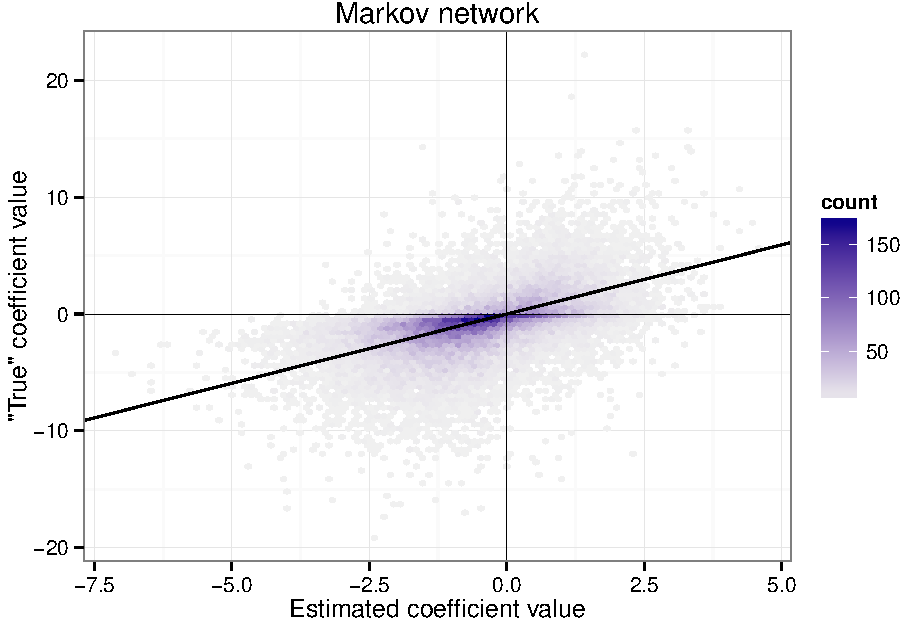
\includegraphics{show-results_files/figure-latex/unnamed-chunk-8-1.png}

\section{C: Inferential statistics}\label{c-inferential-statistics}

\subsection{Identify statistical significance for the Markov network and
Pairs}\label{identify-statistical-significance-for-the-markov-network-and-pairs}

For Pairs, compare the Z-scores with Gaussian quantiles for 95\%
coverage; for the Markov network, use the approximate confidence
intervals estimated in Appendix 3.

\begin{Shaded}
\begin{Highlighting}[]
\NormalTok{pairs_summary =}\StringTok{ }\NormalTok{x[x$method ==}\StringTok{ "null"} \NormalTok{&}\StringTok{ }\NormalTok{!}\KeywordTok{grepl}\NormalTok{(}\StringTok{"pop"}\NormalTok{, x$rep_name), ]}
\NormalTok{markov_summary =}\StringTok{ }\NormalTok{x[x$method ==}\StringTok{ "Markov network"} \NormalTok{&}\StringTok{ }\NormalTok{!}\KeywordTok{grepl}\NormalTok{(}\StringTok{"pop"}\NormalTok{, x$rep_name), ]}


\CommentTok{# Pairs's Z score is based on C-scores, which are positive when species are }
\CommentTok{# disaggregated.  So significantly negative scores imply positive interactions}
\CommentTok{# and vice versa}
\NormalTok{pairs_summary$sig_pos =}\StringTok{ }\NormalTok{pairs_summary$estimate <}\StringTok{ }\KeywordTok{qnorm}\NormalTok{(.}\DecValTok{025}\NormalTok{)}
\NormalTok{pairs_summary$sig_neg =}\StringTok{ }\NormalTok{pairs_summary$estimate >}\StringTok{ }\KeywordTok{qnorm}\NormalTok{(.}\DecValTok{975}\NormalTok{)}

\CommentTok{# Markov network is significant when lower bound is above zero or lower bound is}
\CommentTok{# below zero}
\NormalTok{markov_summary$sig_pos =}\StringTok{ }\NormalTok{markov_summary$lower >}\StringTok{ }\DecValTok{0}
\NormalTok{markov_summary$sig_neg =}\StringTok{ }\NormalTok{markov_summary$upper <}\StringTok{ }\DecValTok{0}
\end{Highlighting}
\end{Shaded}

The \texttt{error\_smoother} is a function that fits a generalized
additive model to estimate the probability that a model estimate will
match some criterion (e.g. statistical significance) for some parameter
as a function of that parameter's ``true'' value. This function is used
in Figure 4C and in calculating Type I error rates below.

\begin{Shaded}
\begin{Highlighting}[]
\NormalTok{truth_seq =}\StringTok{ }\KeywordTok{seq}\NormalTok{(}\KeywordTok{min}\NormalTok{(markov_summary$truth), }\KeywordTok{max}\NormalTok{(markov_summary$truth), }\DataTypeTok{length =} \DecValTok{1000}\NormalTok{)}

\NormalTok{error_smoother =}\StringTok{ }\NormalTok{function(data, f, }\DataTypeTok{values =} \NormalTok{truth_seq)\{}
  \KeywordTok{predict}\NormalTok{(}
    \KeywordTok{gam}\NormalTok{(}
      \KeywordTok{f}\NormalTok{(data) ~}\StringTok{ }\KeywordTok{s}\NormalTok{(truth),}
      \DataTypeTok{data =} \NormalTok{data,}
      \DataTypeTok{family =} \NormalTok{binomial}
    \NormalTok{),}
    \KeywordTok{data.frame}\NormalTok{(}\DataTypeTok{truth =} \NormalTok{values),}
    \DataTypeTok{type =} \StringTok{"response"}
  \NormalTok{)}
\NormalTok{\}}
\end{Highlighting}
\end{Shaded}

\subsection{Create Figure 4}\label{create-figure-4}

Panels A and B plot the point estimates or test statistics for different
models against one another.

Panel C shows the probability of rejecting the null hypothesis (of no
interaction between two species) in the opposite direction of the true
value (see main text).

\begin{Shaded}
\begin{Highlighting}[]
\KeywordTok{pdf}\NormalTok{(}\StringTok{"manuscript-materials/figures/error_rates.pdf"}\NormalTok{, }\DataTypeTok{height =} \FloatTok{8.5}\NormalTok{, }\DataTypeTok{width =} \FloatTok{8.5}\NormalTok{/}\DecValTok{3}\NormalTok{)}
\KeywordTok{par}\NormalTok{(}\DataTypeTok{mfrow =} \KeywordTok{c}\NormalTok{(}\DecValTok{3}\NormalTok{, }\DecValTok{1}\NormalTok{))}

\CommentTok{# Calculate p(confidently wrong) for each model as a function of}
\CommentTok{# the true values}
\NormalTok{confidently_wrong =}\StringTok{ }\NormalTok{function(data)\{}
  \NormalTok{(data$sig_pos &}\StringTok{ }\NormalTok{data$truth <}\StringTok{ }\DecValTok{0}\NormalTok{) |}\StringTok{ }\NormalTok{(data$sig_neg &}\StringTok{ }\NormalTok{data$truth >}\StringTok{ }\DecValTok{0}\NormalTok{)}
\NormalTok{\}}
\NormalTok{y_markov =}\StringTok{ }\KeywordTok{error_smoother}\NormalTok{(markov_summary, confidently_wrong)}
\NormalTok{y_pairs =}\StringTok{ }\KeywordTok{error_smoother}\NormalTok{(pairs_summary, confidently_wrong)}

\CommentTok{# Compare estimates}
\NormalTok{spread_estimates =}\StringTok{ }\NormalTok{x %>%}
\StringTok{  }\NormalTok{dplyr::}\KeywordTok{select}\NormalTok{(-lower, -upper, -X) %>%}
\StringTok{  }\KeywordTok{spread}\NormalTok{(method, estimate) %>%}
\StringTok{  }\KeywordTok{na.omit}\NormalTok{()}

\CommentTok{# R-squared for null versus correlation}
\KeywordTok{round}\NormalTok{(}
  \KeywordTok{summary}\NormalTok{(}\KeywordTok{lm}\NormalTok{(null ~}\StringTok{ }\KeywordTok{I}\NormalTok{(correlation*}\KeywordTok{sqrt}\NormalTok{(n_sites)), }\DataTypeTok{data =} \NormalTok{spread_estimates))$r.squared, }
  \DecValTok{2}
\NormalTok{)}
\end{Highlighting}
\end{Shaded}

\begin{verbatim}
## [1] 0.95
\end{verbatim}

\begin{Shaded}
\begin{Highlighting}[]
\CommentTok{# R-squared for glm markov network versus glm}
\KeywordTok{round}\NormalTok{(}\KeywordTok{summary}\NormalTok{(}\KeywordTok{lm}\NormalTok{(}\StringTok{`}\DataTypeTok{Markov network}\StringTok{`} \NormalTok{~}\StringTok{ }\NormalTok{GLM, }\DataTypeTok{data =} \NormalTok{spread_estimates))$r.squared, }\DecValTok{2}\NormalTok{)}
\end{Highlighting}
\end{Shaded}

\begin{verbatim}
## [1] 0.94
\end{verbatim}

\begin{Shaded}
\begin{Highlighting}[]
\KeywordTok{with}\NormalTok{(}
  \NormalTok{spread_estimates, }
  \KeywordTok{plot}\NormalTok{(}
    \StringTok{`}\DataTypeTok{Markov network}\StringTok{`}\NormalTok{, }
    \NormalTok{GLM, }
    \DataTypeTok{pch =} \StringTok{"."}\NormalTok{, }
    \DataTypeTok{col =} \StringTok{"#00000020"}\NormalTok{,}
    \DataTypeTok{ylab =} \StringTok{"Markov network estimate"}\NormalTok{,}
    \DataTypeTok{xlab =} \StringTok{"GLM estimate"}\NormalTok{,}
    \DataTypeTok{bty =} \StringTok{"l"}
  \NormalTok{)}
\NormalTok{)}
\KeywordTok{mtext}\NormalTok{(}\StringTok{"A. Markov network estimates}\CharTok{\textbackslash{}n}\StringTok{vs. GLM estimates"}\NormalTok{, }\DataTypeTok{adj =} \DecValTok{0}\NormalTok{, }\DataTypeTok{side =} \DecValTok{3}\NormalTok{, }
      \DataTypeTok{font =} \DecValTok{2}\NormalTok{, }\DataTypeTok{line =} \FloatTok{1.2}\NormalTok{, }\DataTypeTok{cex =} \NormalTok{.}\DecValTok{9}\NormalTok{) }
\KeywordTok{abline}\NormalTok{(}\KeywordTok{lm}\NormalTok{(}\StringTok{`}\DataTypeTok{Markov network}\StringTok{`} \NormalTok{~}\StringTok{ }\NormalTok{GLM, }\DataTypeTok{data =} \NormalTok{spread_estimates))}
\KeywordTok{text}\NormalTok{(}\DecValTok{0}\NormalTok{, }\DecValTok{5}\NormalTok{, }\KeywordTok{expression}\NormalTok{(R^}\DecValTok{2}\NormalTok{==}\FloatTok{0.94}\NormalTok{))}

\KeywordTok{with}\NormalTok{(}
  \NormalTok{spread_estimates, }
  \KeywordTok{plot}\NormalTok{(}
    \NormalTok{correlation *}\StringTok{ }\KeywordTok{sqrt}\NormalTok{(n_sites), }
    \NormalTok{null, }
    \DataTypeTok{pch =} \StringTok{"."}\NormalTok{, }
    \DataTypeTok{col =} \StringTok{"#00000020"}\NormalTok{,}
    \DataTypeTok{ylab =} \StringTok{"Z-score"}\NormalTok{,}
    \DataTypeTok{xlab =} \KeywordTok{expression}\NormalTok{(}\StringTok{"correlation"} \NormalTok\StringTok{ }\KeywordTok{sqrt}\NormalTok{(number~}\ErrorTok{~}\NormalTok{of~}\ErrorTok{~}\NormalTok{sites)),}
    \DataTypeTok{bty =} \StringTok{"l"}
  \NormalTok{)}
\NormalTok{)}
\KeywordTok{mtext}\NormalTok{(}\StringTok{"B. Null model estimates vs.}\CharTok{\textbackslash{}n}\StringTok{scaled correlation coefficients"}\NormalTok{, }
      \DataTypeTok{adj =} \DecValTok{0}\NormalTok{, }\DataTypeTok{side =} \DecValTok{3}\NormalTok{, }\DataTypeTok{font =} \DecValTok{2}\NormalTok{, }\DataTypeTok{line =} \FloatTok{1.2}\NormalTok{, }\DataTypeTok{cex =} \NormalTok{.}\DecValTok{9}\NormalTok{) }
\KeywordTok{abline}\NormalTok{(}\KeywordTok{lm}\NormalTok{(null ~}\StringTok{ }\KeywordTok{I}\NormalTok{(correlation*}\KeywordTok{sqrt}\NormalTok{(n_sites)), }\DataTypeTok{data =} \NormalTok{spread_estimates))}
\KeywordTok{text}\NormalTok{(}\DecValTok{10}\NormalTok{, }\DecValTok{12}\NormalTok{, }\KeywordTok{expression}\NormalTok{(R^}\DecValTok{2}\NormalTok{==}\FloatTok{0.95}\NormalTok{))}

\KeywordTok{plot}\NormalTok{(}
  \NormalTok{truth_seq,}
  \NormalTok{y_pairs,}
  \DataTypeTok{type =} \StringTok{"l"}\NormalTok{,}
  \DataTypeTok{xlab =} \StringTok{"}\CharTok{\textbackslash{}"}\StringTok{True}\CharTok{\textbackslash{}"}\StringTok{ interaction strength"}\NormalTok{,}
  \DataTypeTok{ylab =} \StringTok{"P(confidently predict wrong sign)"}\NormalTok{,}
  \DataTypeTok{bty =} \StringTok{"l"}\NormalTok{,}
  \DataTypeTok{yaxs =} \StringTok{"i"}\NormalTok{,}
  \DataTypeTok{col =} \DecValTok{2}\NormalTok{,}
  \DataTypeTok{ylim =} \KeywordTok{c}\NormalTok{(}\DecValTok{0}\NormalTok{, .}\DecValTok{4}\NormalTok{),}
  \DataTypeTok{lwd =} \DecValTok{2}
\NormalTok{)}
\KeywordTok{mtext}\NormalTok{(}\StringTok{"C. Error rate vs.}\CharTok{\textbackslash{}n}\StringTok{interaction strength"}\NormalTok{, }\DataTypeTok{side =} \DecValTok{3}\NormalTok{, }\DataTypeTok{adj =} \DecValTok{0}\NormalTok{, }
      \DataTypeTok{font =} \DecValTok{2}\NormalTok{, }\DataTypeTok{line =} \FloatTok{1.2}\NormalTok{, }\DataTypeTok{cex =} \NormalTok{.}\DecValTok{9}\NormalTok{) }
\KeywordTok{lines}\NormalTok{(truth_seq, y_markov, }\DataTypeTok{lwd =} \DecValTok{2}\NormalTok{)}
\KeywordTok{legend}\NormalTok{(}\StringTok{"topleft"}\NormalTok{, }\DataTypeTok{lwd =} \DecValTok{2}\NormalTok{, }\DataTypeTok{legend =} \KeywordTok{c}\NormalTok{(}\StringTok{"Null model"}\NormalTok{, }\StringTok{"Markov network"}\NormalTok{), }
       \DataTypeTok{col =} \KeywordTok{c}\NormalTok{(}\DecValTok{2}\NormalTok{, }\DecValTok{1}\NormalTok{), }\DataTypeTok{bty =} \StringTok{"n"}\NormalTok{)}
\KeywordTok{dev.off}\NormalTok{()}
\end{Highlighting}
\end{Shaded}

\begin{verbatim}
## pdf 
##   2
\end{verbatim}

\subsection{Summarize inferential
statistics:}\label{summarize-inferential-statistics}

\paragraph{P(Pairs confidently wrong):}\label{ppairs-confidently-wrong}

\begin{Shaded}
\begin{Highlighting}[]
\KeywordTok{with}\NormalTok{(pairs_summary,  }\KeywordTok{mean}\NormalTok{((sig_neg &}\StringTok{ }\NormalTok{truth >}\StringTok{ }\DecValTok{0}\NormalTok{) |}\StringTok{ }\NormalTok{(sig_pos &}\StringTok{ }\NormalTok{truth <}\StringTok{ }\DecValTok{0}\NormalTok{)))}
\end{Highlighting}
\end{Shaded}

\begin{verbatim}
## [1] 0.1533758
\end{verbatim}

\paragraph{P(Markov network confidently
wrong)}\label{pmarkov-network-confidently-wrong}

\begin{Shaded}
\begin{Highlighting}[]
\KeywordTok{with}\NormalTok{(markov_summary, }\KeywordTok{mean}\NormalTok{((sig_neg &}\StringTok{ }\NormalTok{truth >}\StringTok{ }\DecValTok{0}\NormalTok{) |}\StringTok{ }\NormalTok{(sig_pos &}\StringTok{ }\NormalTok{truth <}\StringTok{ }\DecValTok{0}\NormalTok{)))}
\end{Highlighting}
\end{Shaded}

\begin{verbatim}
## [1] 0.02861541
\end{verbatim}

\paragraph{P(Pairs rejects null)}\label{ppairs-rejects-null}

\begin{Shaded}
\begin{Highlighting}[]
\KeywordTok{with}\NormalTok{(pairs_summary,  }\KeywordTok{mean}\NormalTok{(sig_neg |}\StringTok{ }\NormalTok{sig_pos))}
\end{Highlighting}
\end{Shaded}

\begin{verbatim}
## [1] 0.4520535
\end{verbatim}

\paragraph{P(Markov network rejects
null)}\label{pmarkov-network-rejects-null}

\begin{Shaded}
\begin{Highlighting}[]
\KeywordTok{with}\NormalTok{(markov_summary,  }\KeywordTok{mean}\NormalTok{(sig_neg |}\StringTok{ }\NormalTok{sig_pos))}
\end{Highlighting}
\end{Shaded}

\begin{verbatim}
## [1] 0.2116561
\end{verbatim}

\subsection{Type I error rates:}\label{type-i-error-rates}

Type I error rates (probability of rejecting the null hypothesis given a
``true'' interaction strength of zero, according to the spline model
defined by \texttt{error\_smoother} above). The smoother focuses on the
64\% of the data points whose ``true'' values fall between -1 and 1,
because its estimates near 0 are more accurate when they aren't affected
by distant data points.

\paragraph{Markov network Type I error
rates}\label{markov-network-type-i-error-rates}

\begin{Shaded}
\begin{Highlighting}[]
\NormalTok{markov_summary %>%}\StringTok{ }
\StringTok{  }\KeywordTok{filter}\NormalTok{(}\KeywordTok{abs}\NormalTok{(truth) <}\StringTok{ }\DecValTok{1}\NormalTok{) %>%}\StringTok{ }
\StringTok{  }\KeywordTok{group_by}\NormalTok{(simulation_type) %>%}\StringTok{ }
\StringTok{  }\KeywordTok{do}\NormalTok{(}\KeywordTok{data.frame}\NormalTok{(}
    \StringTok{`}\DataTypeTok{Type I error rate}\StringTok{`} \NormalTok{=}\StringTok{ }
\StringTok{      }\KeywordTok{error_smoother}\NormalTok{(., function(x)\{x$sig_pos |}\StringTok{ }\NormalTok{x$sig_neg\}, }\DataTypeTok{values =} \DecValTok{0}\NormalTok{)}
  \NormalTok{)) %>%}
\StringTok{  }\KeywordTok{kable}\NormalTok{(}\DataTypeTok{digits =} \DecValTok{3}\NormalTok{)}
\end{Highlighting}
\end{Shaded}

\begin{longtable}[c]{@{}lr@{}}
\toprule
simulation\_type & Type.I.error.rate\tabularnewline
\midrule
\endhead
abund & 0.258\tabularnewline
env & 0.142\tabularnewline
no\_env & 0.024\tabularnewline
\bottomrule
\end{longtable}

\paragraph{Null model Type I error
rates}\label{null-model-type-i-error-rates}

\begin{Shaded}
\begin{Highlighting}[]
\NormalTok{pairs_summary %>%}\StringTok{ }
\StringTok{  }\KeywordTok{filter}\NormalTok{(}\KeywordTok{abs}\NormalTok{(truth) <}\StringTok{ }\DecValTok{1}\NormalTok{) %>%}\StringTok{ }
\StringTok{  }\KeywordTok{group_by}\NormalTok{(simulation_type) %>%}\StringTok{ }
\StringTok{  }\KeywordTok{do}\NormalTok{(}\KeywordTok{data.frame}\NormalTok{(}
    \StringTok{`}\DataTypeTok{Type I error rate}\StringTok{`} \NormalTok{=}\StringTok{ }
\StringTok{      }\KeywordTok{error_smoother}\NormalTok{(., function(x)\{x$sig_pos |}\StringTok{ }\NormalTok{x$sig_neg\}, }\DataTypeTok{values =} \DecValTok{0}\NormalTok{)}
  \NormalTok{)) %>%}
\StringTok{  }\KeywordTok{kable}\NormalTok{(}\DataTypeTok{digits =} \DecValTok{3}\NormalTok{)}
\end{Highlighting}
\end{Shaded}

\begin{longtable}[c]{@{}lr@{}}
\toprule
simulation\_type & Type.I.error.rate\tabularnewline
\midrule
\endhead
abund & 0.597\tabularnewline
env & 0.530\tabularnewline
no\_env & 0.308\tabularnewline
\bottomrule
\end{longtable}

\subsection{\texorpdfstring{Plot Markov network confidence interval
coverage versus true \(\beta\)
value}{Plot Markov network confidence interval coverage versus true \textbackslash{}beta value}}\label{plot-markov-network-confidence-interval-coverage-versus-true-beta-value}

The top and bottom 0.5\% of the distribution have been omitted to
prevent bad behavior by the smoother in the tails. The horizontal red
line shows the nominal 95\% coverage rate and the black vertical line
marks where the ``true'' value of \(\beta\) was zero. The Type I error
rates calculated above for the Markov network closely match (one minus)
the values of these curves at zero.

\begin{Shaded}
\begin{Highlighting}[]
\NormalTok{coverage_data =}\StringTok{ }\NormalTok{markov_summary %>%}
\StringTok{  }\KeywordTok{filter}\NormalTok{(}\KeywordTok{percent_rank}\NormalTok{(truth) >}\StringTok{ }\NormalTok{.}\DecValTok{005} \NormalTok{&}\StringTok{ }\KeywordTok{percent_rank}\NormalTok{(truth) <}\StringTok{ }\NormalTok{.}\DecValTok{995}\NormalTok{) %>%}
\StringTok{  }\KeywordTok{mutate}\NormalTok{(}\DataTypeTok{covered =} \NormalTok{truth >}\StringTok{ }\NormalTok{lower &}\StringTok{ }\NormalTok{truth <}\StringTok{ }\NormalTok{upper) %>%}
\StringTok{  }\KeywordTok{mutate}\NormalTok{(}\DataTypeTok{simulation_type =} \KeywordTok{factor}\NormalTok{(simulation_type, }\KeywordTok{c}\NormalTok{(}\StringTok{"no_env"}\NormalTok{, }\StringTok{"env"}\NormalTok{, }\StringTok{"abund"}\NormalTok{)))}

\KeywordTok{ggplot}\NormalTok{(coverage_data, }\KeywordTok{aes}\NormalTok{(}\DataTypeTok{x =} \NormalTok{truth, }\DataTypeTok{y =} \KeywordTok{as.integer}\NormalTok{(covered))) +}\StringTok{ }
\StringTok{  }\KeywordTok{facet_grid}\NormalTok{(~simulation_type) +}\StringTok{ }
\StringTok{  }\KeywordTok{geom_smooth}\NormalTok{(}\DataTypeTok{method =} \NormalTok{gam, }\DataTypeTok{formula =} \NormalTok{y ~}\StringTok{ }\KeywordTok{s}\NormalTok{(x), }\DataTypeTok{method.args =} \KeywordTok{list}\NormalTok{(}\DataTypeTok{family =} \NormalTok{binomial)) +}\StringTok{ }
\StringTok{  }\KeywordTok{theme_bw}\NormalTok{() +}\StringTok{ }
\StringTok{  }\KeywordTok{coord_cartesian}\NormalTok{(}\DataTypeTok{ylim =} \KeywordTok{c}\NormalTok{(}\DecValTok{0}\NormalTok{, }\DecValTok{1}\NormalTok{), }\DataTypeTok{expand =} \OtherTok{FALSE}\NormalTok{) +}\StringTok{ }
\StringTok{  }\KeywordTok{geom_vline}\NormalTok{(}\DataTypeTok{xintercept =} \DecValTok{0}\NormalTok{) +}\StringTok{ }
\StringTok{  }\KeywordTok{geom_hline}\NormalTok{(}\DataTypeTok{yintercept =} \FloatTok{0.95}\NormalTok{, }\DataTypeTok{color =} \StringTok{"red"}\NormalTok{) +}\StringTok{ }
\StringTok{  }\KeywordTok{ylab}\NormalTok{(}\StringTok{"Coverage"}\NormalTok{)}
\end{Highlighting}
\end{Shaded}

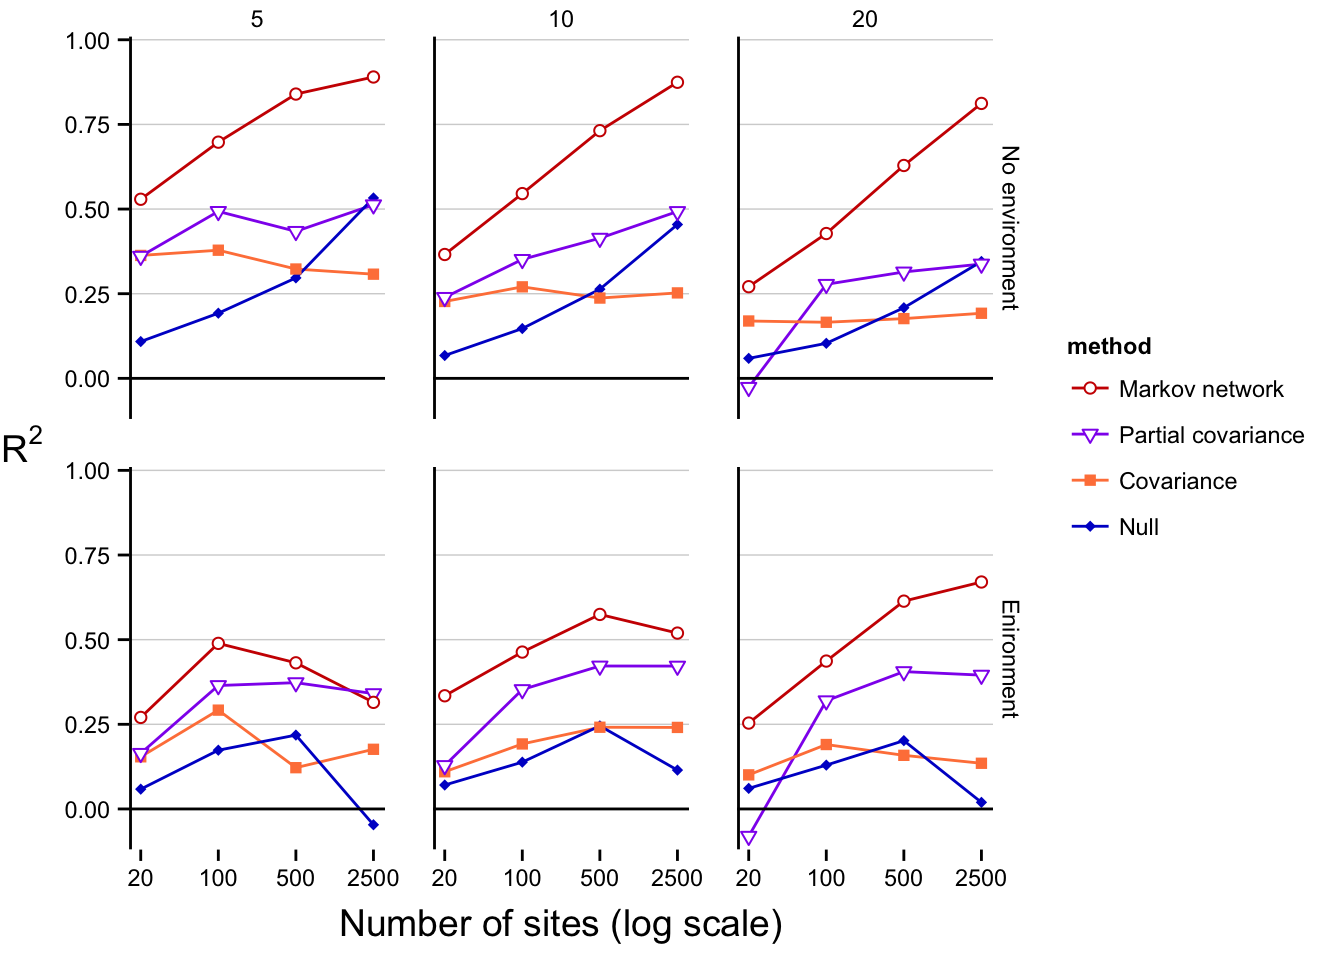
\includegraphics{show-results_files/figure-latex/unnamed-chunk-18-1.pdf}

\end{document}
